\begin{center}
    \section{Семинар XI}
\end{center}
\subsection{Квазиклассика.}
\hspace{1em} Всю первую часть нашего курса мы решали задачи с потенциальными ямами. Решали мы их честно -- решая уравнение Шрёдингера для каждой из областей. Но почти все задачи были модельными -- то и дело приходилось работать с бесконечными стенками, вертикальными барьерами и так далее. На практике же потенциалы совершенно разные, необязательно константные. Для таких потенциалов решать уравнение Шрёдингера становится сильно сложнее. Поэтому для исследования более сложных систем мы начинаем привлекать различные приближённые методы. И первый такой метод -- рассмотрение \textit{квазиклассических} систем. В англоязычной литературе этот подход называется в честь метода аппроксимации, который мы будем использовать -- WKB approximation.

\subsubsection{Классически разрешенные и запрещённые зоны.}
\hspace{1em} Давно мы не писали уравнение Шрёдингера. Исправим это недоразумение:
\[
-\frac{\hbar^2}{2m}\psi''(x) + V(x)\psi = E\psi
\]
Пусть E > V(x), то есть рассматриваемая область классически разрешенная. Будем искать решение этого уравнения в виде $\psi(x) = e^{\frac{i}{\hbar}S(x)}$. В отличие от классических для нас решений, здесь потенциал имеет общий вид, поэтому в экспоненте есть функция, зависящая от x. Подставим волновую функцию такого вида в уравнение:
\[
\frac{1}{2m}(S')^2 - \frac{i\hbar}{2m}S'' = E - V(x)
\]
Чтобы продолжить решение этого уравнения, необходимо воспользоваться тем самым квазиклассическим приближением. 

В классике $\hbar \rightarrow 0$, поэтому мы можем разложить функцию $S(x)$ по степеням $\hbar$ и, включая в решение всё более высокую степень $\hbar$, управлять точностью решения уравнения. Таким образом:
\[
S(x) = S_0 + \hbar S_1 + \hbar^2 S_2 + ...
\]
Для получения важных результатов нам достаточно взять два первых члена. Подставим их в левую часть уравнения и получим:
\[
\frac{1}{2m}\left( S'_0 + \hbar S'_1 \right)^2 - \frac{i\hbar}{2m}(S''_0 + \hbar S''_1) = \frac{1}{2m}\left( (S'_0)^2 + 2\hbar S'_0 S'_1 + \hbar^2 (S'_1)^2 \right) - \frac{i\hbar}{2m}(S''_0 + \hbar S''_1)
\]
Выделим члены при $\hbar^0 = 1$. Добавив правую часть уравнения, получим:
\[
\frac{1}{2m}(S'_0)^2 = E - V(x)
\]
Это простое дифференциальное уравнение с разделяющимися переменными. Решением будет:
\[
S_0(x) = \pm \int\sqrt{2m\left( E - V(x) \right)}dx = \int p(x)dx,
\]
где функция p(x) -- классический импульс. 

В первом приближении мы получаем классическое действие. Это логично -- мы отбрасываем квантовый множитель, получая чисто классическое уравнение. Условие для использования такого приближения можно записать в виде $\hbar|S''/(S')^2| \ll 1$. Если подставить $S' = p$, получим
\[
|\frac{d\lambda(x)}{dx}| \ll 1, \quad \lambda(x) = \frac{\hbar}{px}
\]

Получается, что условие квазиклассичности -- малое изменение волны де-Бройля. Если говорить проще, то классический импульс частицы не должен становиться слишком маленьким. Такое происходит, например, в точках поворота, когда $V(x) = E$. Мы рассмотрим этот случай чуть позже. Пока давайте найдём решение при учёте первой степени $\hbar$:
\[
\frac{\hbar}{m}S'_0 S'_1 - \frac{i\hbar}{2m}S''_0 = 0 \implies S'_1 = \frac{iS''_0}{2S'_0} = \frac{i}{2}\frac{p'}{p}
\]
Тогда, решая этот диффур, находим:
\[
S_1 = C\frac{i}{2}\ln p
\]

Теперь, подставив найденные значения в исходный вид волновой функции $\psi(x) = e^{\frac{i}{\hbar}(S_0 + \hbar S_1)}$, получим:
\[
\psi(x) \simeq \frac{C_1}{\sqrt{p}}\exp\left(\frac{i}{\hbar}\int p dx \right) + \frac{C_2}{\sqrt{p}}\exp\left(-\frac{i}{\hbar}\int p dx \right)
\]
В запрещённой области импульс будет мнимым (так как E - V(x) < 0), поэтому показатель экспоненты будет вещественным. Волновая функция будет иметь вид:
\[
\psi(x) \simeq \frac{C_1}{\sqrt{|p|}}\exp\left(\frac{1}{\hbar}\int |p| dx \right) + \frac{C_2}{\sqrt{p}}\exp\left(-\frac{1}{\hbar}\int |p| dx \right)
\]
Этих знаний уже достаточно, чтобы рассмотреть какой-нибудь простенький потенциал.
\excersize{Упражнение №34}{darklavender}
\begin{center}
    \textit{Используя квазиклассическое приближение, найдите энергию и волновые функции, представленного на рисунке \ref{fig 11.1}.}
    \[
    V(x) = 
    \begin{cases}
    \text{какая-то функция, } 0<x<a\\
    +\infty, \text{в другом случае}
    \end{cases}
    \]
\end{center}

\begin{figure}[ht]
\centering
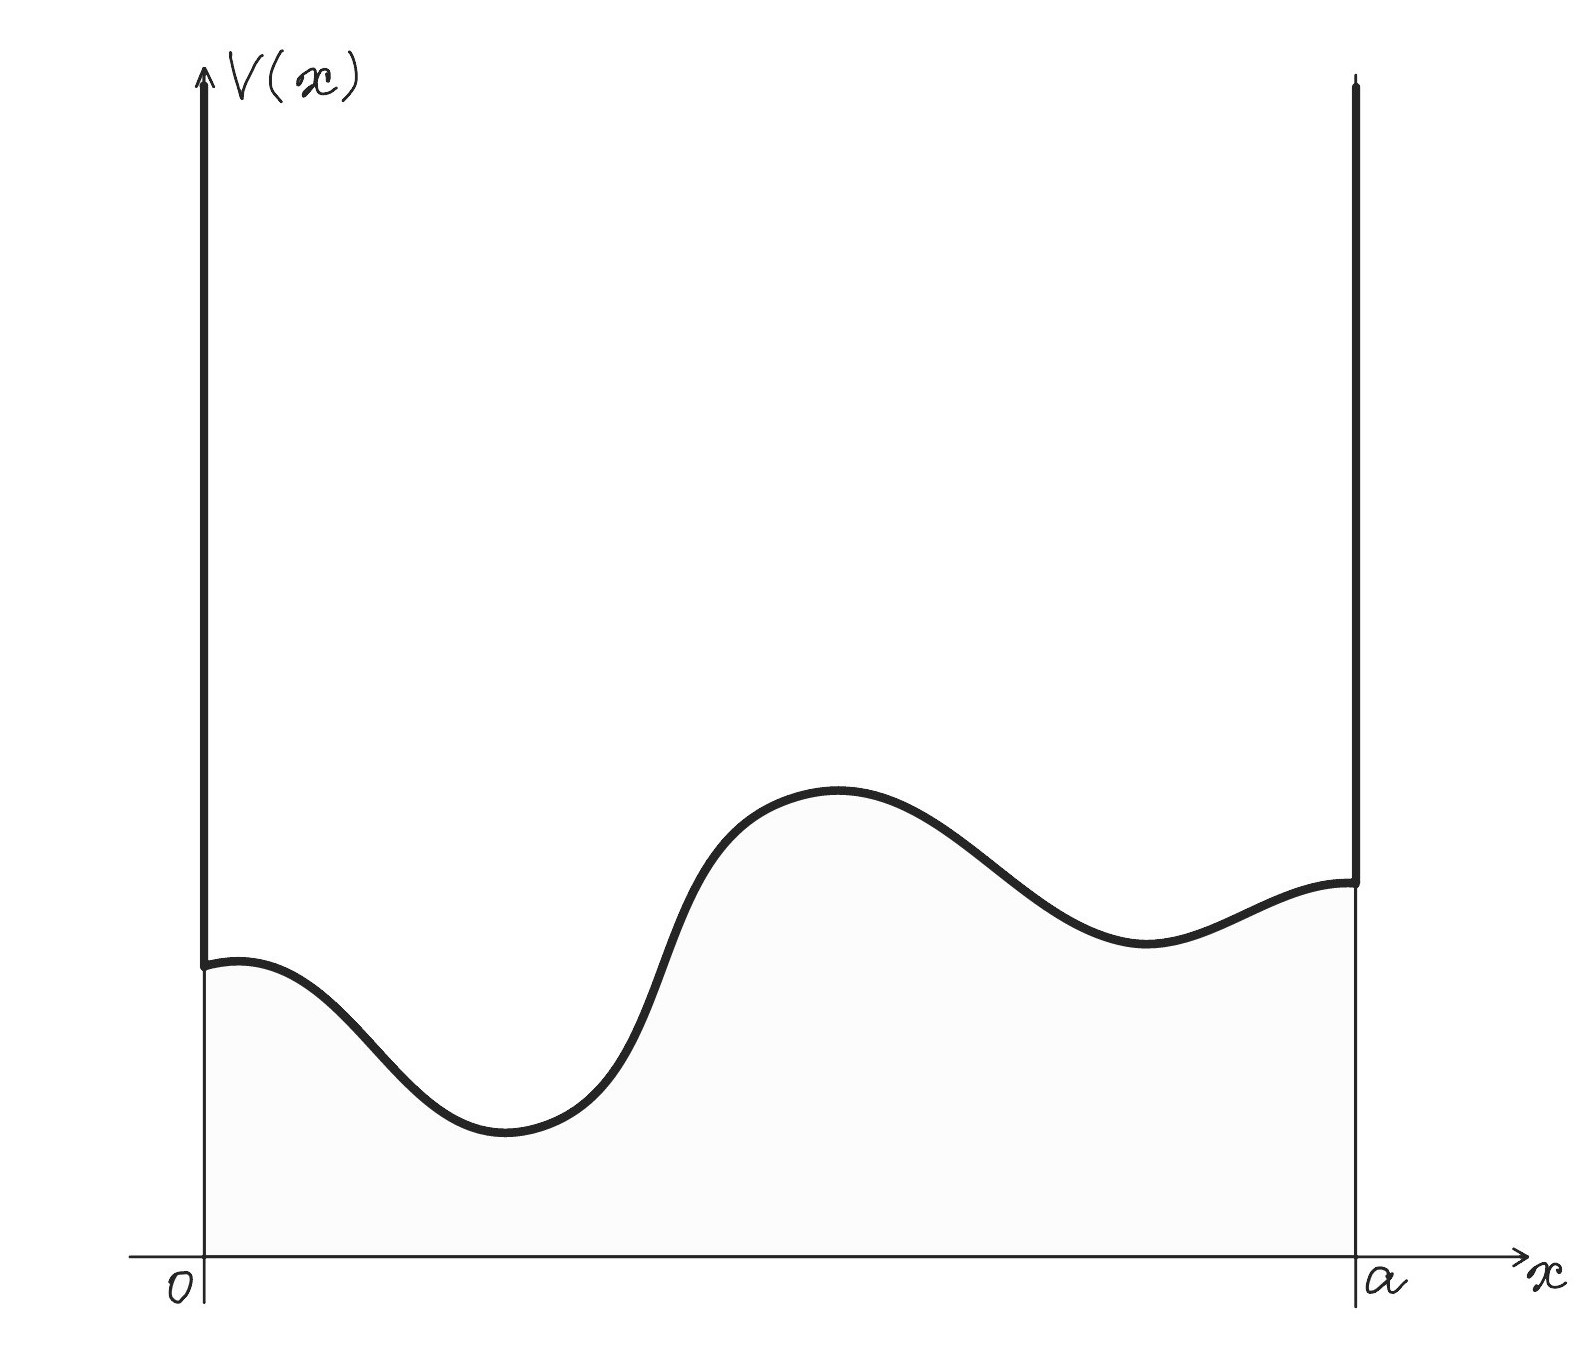
\includegraphics[scale=0.2]{class_11/images/bound-state.jpg}
\caption{Какое-то связанное состояние}
\label{fig 11.1}
\end{figure}

Мы уже решали похожую задачу, однако здесь мы имеем какое-то произвольное дно. Для нас самое главное, чтобы на нём не было резких изменений -- тогда условия квазиклассичности будут соблюдены.

Волновая функция за стенками, очевидно, равна нулю. Внутри ящика мы воспользуемся полученными выражениями:
\[
\psi(x) \simeq \frac{\widetilde{C}_1}{\sqrt{p}}e^{\frac{i}{\hbar}S(x)} + \frac{\widetilde{C}_2}{\sqrt{p}}e^{-\frac{i}{\hbar}S(x)} = \frac{C_1}{\sqrt{p}}\sin (\frac{S(x)}{\hbar}) + \frac{C_2}{\sqrt{p}}\cos(\frac{S(x)}{\hbar}),
\]
где $S(x) = \int\limits_{0}^{x}p\, dx'$. Так как $\psi(0) = 0$, получим, что $C_2 = 0$ (так как $S(0) = 0$). В точке $a$ волновая функция $\psi(a) = 0$, значит $S(a) = \pi n$, $n = 0, 1, 2, ...$. Тогда
\[
\int\limits_{0}^{a}p\, dx = \pi n \hbar
\]
С помощью этого выражения можно находить приближённые значения энергии. Давайте посмотрим на случай, когда дно ровное (то есть V(x)=0 -- константная функция). В таком случае интеграл от импульса равен $\int\limits_{0}^{a}p\, dx = \int\limits_{0}^{a}\sqrt{2mE} = a\sqrt{2mE}$. Подставляя его в полученное выражение, выразим энергию:
\[
E = \frac{n^2\pi^2\hbar^2}{2ma^2}
\]
Результат получился такой же, как и при честном решении уравнения Шрёдингера. Это отлично!
\csquare{darklavender}

\begin{figure}[ht]
\centering
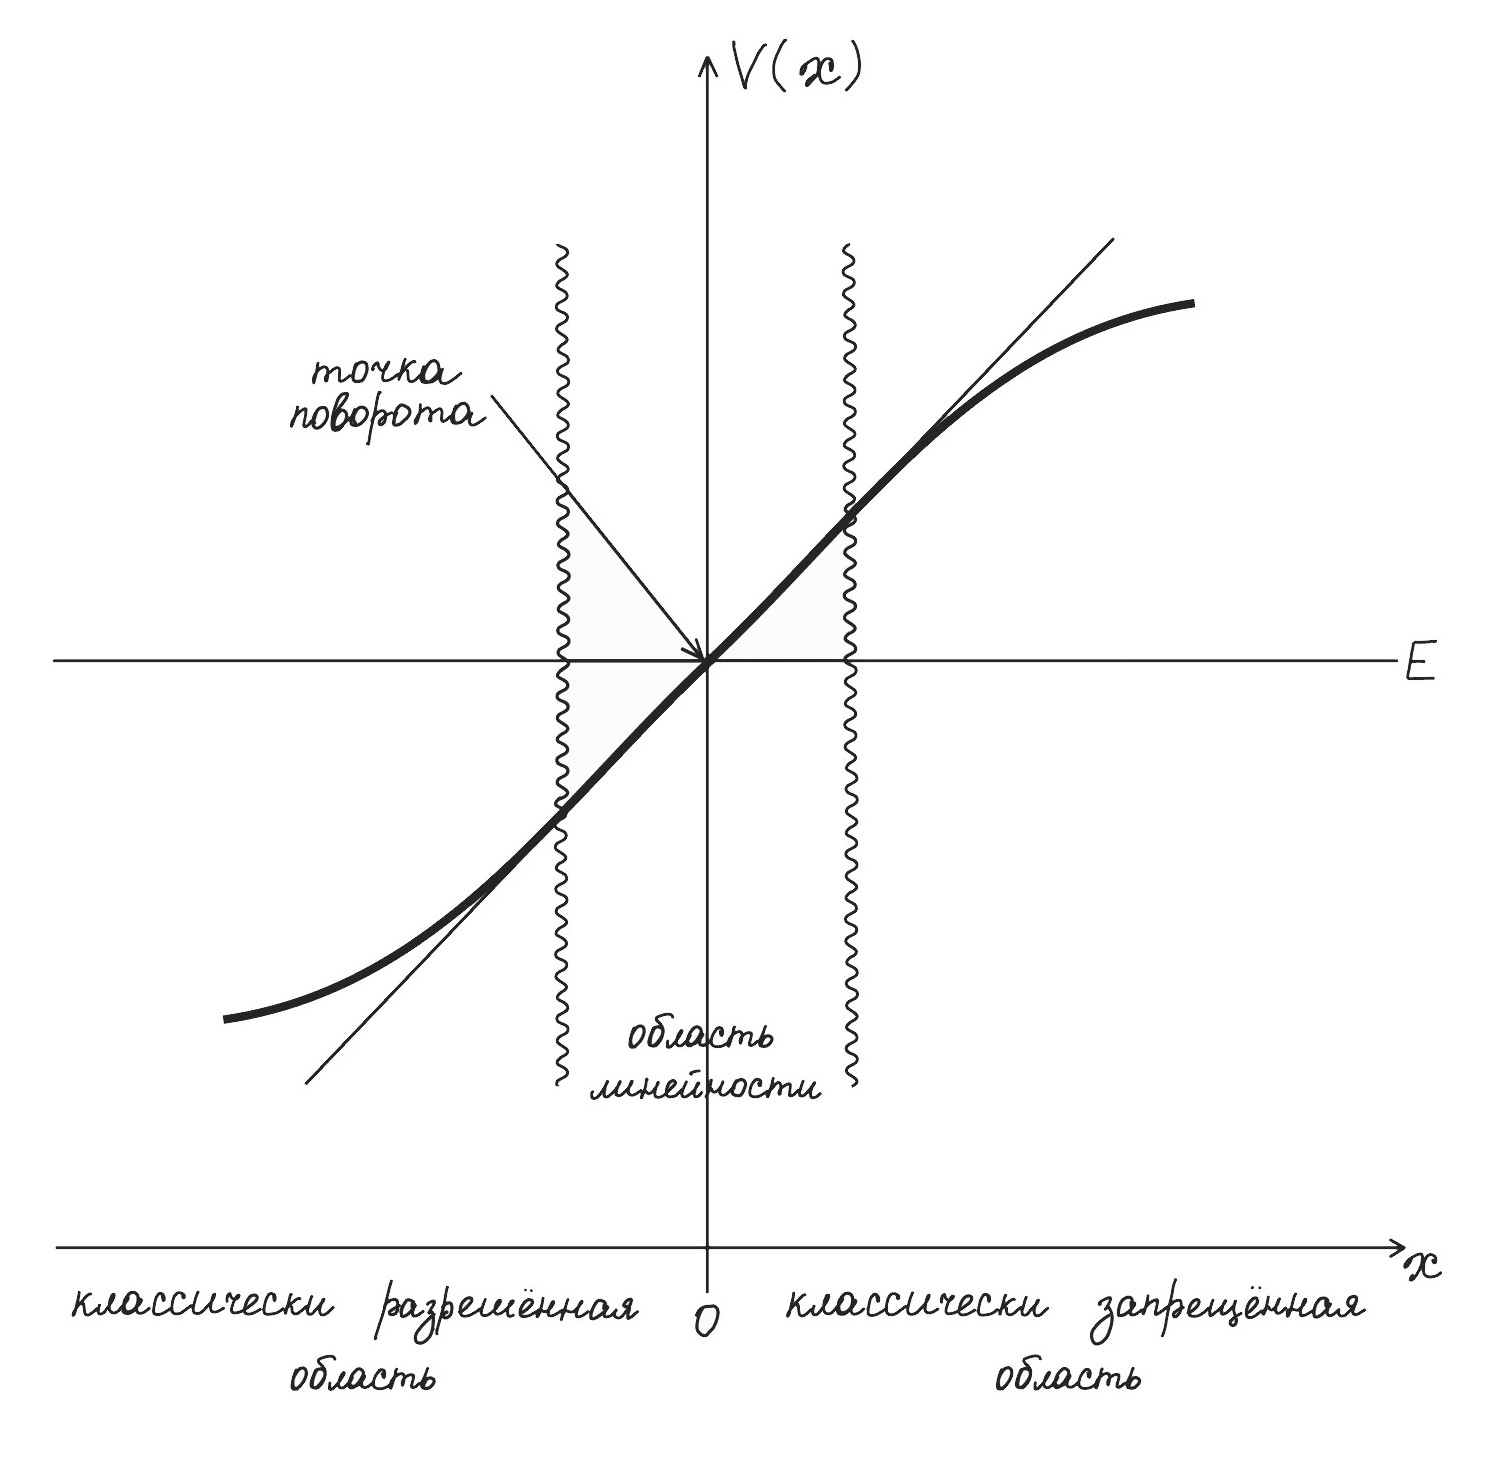
\includegraphics[scale=0.28]{class_11/images/turning-point.jpg}
\caption{Линейное приближение потенциала.}
\label{fig 11.2}
\end{figure}

Теперь эти два решения нужно каким-то образом объединить. Сложность здесь состоит в том, что вблизи точек поворота импульс частицы в классическом случае стремится к нулю и применение квазиклассического приближения становится невозможным. Поэтому приходиться решать уравнение Шрёдингера ``честно''.\footnote{Здесь, в отличие от Ландау, я не буду уходить в ``методически более поучительный'' вариант, так как он привлекает знания ТФКП, которых после сдачи экзамена остаётся не так уж и много. Давайте лучше решать диффуры, это у нас хорошо получается.} Так как мы рассматриваем потенциал достаточно близко к точкам поворота (см. рисунок \ref{fig 11.2}), давайте аппроксимируем наш потенциал прямой линией, используя разложение Тейлора:
\[
V(x) \simeq E + V'(0)x,\; E = V(0)
\]
Подставим этот потенциал в уравнение Шрёдингера:
\[
-\frac{\hbar^2}{2m}\frac{d^2 \psi_T}{dx^2} + [E + V'(0)x]\psi_T = E\psi_T
\]
или
\[
\frac{d^2 \psi_T}{dx^2} = \alpha^3 x \psi_T, \, \alpha = \left[ \frac{2m}{\hbar} V'(0) \right]^{1/3}
\]
Здесь я ввёл обозначение $\psi_T$ для уточнения, что это волновая функция в окрестности точки поворота. Тогда, введя новую переменную $z = \alpha x$, получим \textit{уравнение Эйри}:
\[
\frac{d^2 \psi_T}{dz^2} = z\psi(x)
\]
Решением этого уравнение будут функции Эйри:
\[
\psi_T(x) = aAi(z) + bBi(z)
\]
Подробнее про решение этого уравнения и сами функции можно почитать в третьем томе Ландау, в математических дополнениях. Я не буду вдаваться в это слишком подробно, выпишу лишь основные свойства функций, которые нам понадобятся.

Интегральный вид функций Эйри:
\[
Ai(z) = \frac{1}{\pi}\int\limits_{0}^{\infty}\cos(\frac{s^3}{3} + sz)ds; \quad Bi(z) = \frac{1}{\pi}\int\limits_{0}^{\infty}\left[e^{\frac{-s^3}{3} + sz} + \sin(\frac{s^3}{3} + sz)\right]ds;
\]

Асимптотики:
\[
\begin{rcases}
    Ai(z) \sim \frac{1}{2\sqrt{\pi}z^{1/4}}e^{-\frac{2}{3}z^{3/2}}\\
    Bi(z) \sim \frac{1}{\sqrt{\pi}z^{1/4}}e^{\frac{2}{3}z^{3/2}}
\end{rcases}
 z \gg 0;\quad
 \begin{rcases}
    Ai(z) \sim \frac{1}{\sqrt{\pi}(-z)^{1/4}}\sin\left[\frac{2}{3}(-z)^{3/2} + \frac{\pi}{4}\right]\\
    Bi(z) \sim \frac{1}{\sqrt{\pi}(-z)^{1/4}}\cos\left[\frac{2}{3}(-z)^{3/2} + \frac{\pi}{4}\right]
\end{rcases}
z\ll 0
\]

Теперь мы знаем, как выглядит волновая функция, которая поможет нам объединить две области -- классически запрещённую (слева) и классически разрешенную (справа). Найдём волновую функцию справа. Сначала запишем общий вид волновой функции вне области точки поворота. 
\[
\psi(x) \simeq
\begin{cases}
    \frac{1}{\sqrt{p}}\left[B\exp\left(\frac{i}{\hbar}\int\limits_x^{0}p dx'\right) + C\exp\left(-\frac{i}{\hbar}\int\limits_x^{0}p dx'\right)\right],\; \text{при } x < 0\\
    \frac{1}{\sqrt{|p|}}\left[D\exp\left(-\frac{1}{\hbar}\int\limits_0^{x}|p| dx'\right)\right],\; \text{при } x > 0
\end{cases}
\]

Возьмём область достаточно далёкую от точки поворота, чтобы можно было воспользоваться квазиклассическим приближением, и при этом достаточно близкую, чтобы потенциал был линейный. Тогда:
\[
p(x) \simeq \sqrt{2m (E - E - V'(0)x)} = \hbar\alpha^{3/2}\sqrt{-x}
\]
Для запрещённой области будет выполняться:
\[
\int\limits_{0}^{x}|p|dx' \simeq \hbar\alpha^{3/2}\int\limits_{0}^{x} \sqrt{x'}dx' = \frac{2}{3}\hbar(\alpha x)^{3/2}
\]
Подставляя это в волновую функцию, получим:
\[
\psi(x) \simeq \frac{D}{\sqrt{\hbar}\alpha^{3/4}x^{1/4}}e^{-\frac{2}{3}(\alpha x)^{3/2}}
\]
Возвращаясь к волновой функции у точки поворота, воспользуемся асимптотикой для больших значений z\footnote{Возможность использовать такую аппроксимацию может показаться странной, так как при z=0 мы находимся к точке поворота очень близко. Но, на практике, такое решение имеет место, так как и значение $\alpha x$ достаточно большое, и потенциал ещё линейный. Конкретные значения можно увидеть в \nameref{appendix:C} в первой задаче.}. Тогда её вид в правой области будет следующий:
\[
\psi_T \simeq \frac{a}{2\sqrt{\pi} (\alpha x)^{1/4}}e^{-\frac{2}{3}(\alpha x)^{3/2}} +  \frac{b}{\sqrt{\pi} (\alpha x)^{1/4}}e^{\frac{2}{3}(\alpha x)^{3/2}}
\]
Сравнивая эти волновые функции, мы видим:
\[
a = \sqrt{\frac{4\pi}{\alpha \hbar}}D, \quad b = 0
\]
Проделаем то же самое с областью слева. Посчитаем интеграл от импульса, не забывая, что x теперь отрицательный:
\[
\int\limits_{x}^{0}p\, dx' \simeq \frac{2}{3}\hbar(-\alpha x)^{3/2}
\]
Подставляем в волновую функцию для классически разрешенной области:
\[
\psi(x) \simeq \frac{1}{\sqrt{\hbar}\alpha^{3/4}(-x)^{1/4}}\left[Be^{i\frac{2}{3}(-\alpha x)^{3/2}}+ Ce^{-i\frac{2}{3}(-\alpha x)^{3/2}}\right]
\]
Снова используем асимптотику, но теперь z -- большое отрицательное число, значит и асимптотика будет для $z\ll 0$. Также учитываем, что мы уже нашли коэффициент b -- он равен нулю. Теперь, когда мы ничего не забыли, пишем:
\begin{align*}
\psi_T & \simeq \frac{a}{\sqrt{\pi}(-\alpha x)^{1/4}}\sin\left[\frac{2}{3}(-\alpha x)^{3/2} + \frac{\pi}{4}\right] = \\ & = \frac{a}{\sqrt{\pi}(-\alpha x)^{1/4}}\frac{1}{2i}\left[ e^{i\pi/4}e^{i\frac{2}{3}(-\alpha x)^{3/2}} - e^{-i\pi/4}e^{-i\frac{2}{3}(-\alpha x)^{3/2}}\right]
\end{align*}
Вновь сравнивая функции, получим:
\[
\frac{a}{2i\sqrt{\pi}}e^{i\pi/4} = \frac{B}{\sqrt{\hbar \alpha}}, \quad \frac{-a}{2i\sqrt{\pi}}e^{-i\pi/4} = \frac{C}{\sqrt{\hbar \alpha}},
\]
или, если подставим ранее полученное выражение для $a$:
\[
B = -ie^{i\pi/4}D, \quad C = ie^{-i\pi/4}D
\]
Подставляя эти коэффициенты в первоначальное общее выражение для волновой функции, получим \textit{формулы связи} для области возрастающего потенциала, где $x_2$ -- точка поворота:
\[
\psi_R(x) \simeq 
\begin{cases}
    \frac{2D}{\sqrt{p}}\sin\left[ \frac{1}{\hbar} \int\limits_x^{x_2} p\,dx' + \frac{\pi}{4} \right], \; \text{при } x < x_2\\
    \frac{D}{\sqrt{|p|}}\exp\left[-\frac{1}{\hbar} \int\limits_{x_2}^{x} |p|\,dx' \right],\; \text{при } x > x_2
\end{cases}
\]

Используя тот же самый подход, получим волновую функцию для области убывающего потенциала, где $x_1$ -- точка поворота. Точный расчёт можно посмотреть во второй задаче в \nameref{appendix:C}.
\[
\psi_L(x) \simeq 
\begin{cases}
    \frac{D'}{\sqrt{|p|}}\exp\left[-\frac{1}{\hbar} \int\limits_{x}^{x_1} |p|\,dx' \right],\; \text{при } x < x_1\\
    \frac{2D'}{\sqrt{p}}\sin\left[ \frac{1}{\hbar} \int\limits_{x_1}^{x} p\,dx' + \frac{\pi}{4} \right], \; \text{при } x > x_1\\
\end{cases}
\]

Теперь, когда у нас есть обе волновые функции, вновь рассмотрим потенциальную яму, но теперь у нас нет бесконечных стенок. Рассматривая ``пересекающуюся'' область, волновую функцию для классической области можно записать в виде:
\[
\psi(x) \simeq \frac{2D}{\sqrt{p}}\sin\theta_2(x),\quad \theta_2(x) = \frac{1}{\hbar}\int\limits_{x}^{x_2}p\,dx' + \frac{\pi}{4},
\]
или, используя левую точку поворота:
\[
\psi(x) \simeq \frac{-2D'}{\sqrt{p}}\sin\theta_1(x),\quad \theta_1(x) = -\frac{1}{\hbar}\int\limits_{x_1}^{x}p\,dx' - \frac{\pi}{4}.
\]

Аргументы у синусов должны быть равны по модулю $\pi$, то есть $\theta_2 = \theta_1 + \pi n$. Подставляя полученные выше значения, получим:
\[
\int\limits_{x_1}^{x_2}p\, dx = (n + \frac{1}{2})\hbar\pi,\quad n = 0, 1, 2, ...
\]

Это, так называемое, \textit{правило квантования Бора - Зоммерфельда}. Оно позволяет в случае потенциальных ям с большим значением $n$ найти энергию без решения уравнению Шрёдингера. 

Имея на руках все инструменты, давайте попробуем решить следующую задачу.

\excersize{Упражнение №35}{darklavender}
\begin{center}
    \textit{Найдите энергию и волновые функции для следующих потенциалов:}
    \[
    a)\;V(x) = \frac{m\omega^2 x^2}{2}
    \]
    \[
    b)\;V(x) = 
    \begin{cases}
     \frac{m\omega^2 x^2}{2},\;x > 0\\
    +\infty,\; x < 0
    \end{cases}
    \]
\end{center}

a) Для начала найдём энергию, воспользовавшись правилом Бора-Зоммерфельда. Импульс в нашей задаче равен $p = \sqrt{2mE - m^2\omega^2x^2}$. Точку поворота можно получить, приравняв импульс к нулю и выразив $x$:
\[
x_0 = \sqrt{\frac{2E}{m\omega^2}}
\]
Подставим это в интеграл и посчитаем его:
\begin{align*}
\int\limits_{-x_0}^{x_0}p\;dx & = \int\limits_{-x_0}^{x_0}\sqrt{2mE - m^2\omega^2x^2}\;dx =\\& = \frac{m\omega}{2}\left[x\sqrt{\frac{2E}{m\omega^2}- x^2} + \frac{2E}{m\omega^2}\arctan\left( \frac{x}{\sqrt{\frac{2E}{m\omega^2} - x^2}} \right)\right]\Bigg|_{-x_0}^{x_0} = \\ & = \left( tan^{-1}(+\infty) = \frac{\pi}{2}\right) = 2(\frac{m\omega}{2}\frac{2E}{m\omega^2}\frac{\pi}{2}) = \frac{E\pi}{\omega} = (n + \frac{1}{2})\hbar\pi
\end{align*}
Выражая энергию, получим ожидаемый результат
\[
E_n = \hbar\omega(n + \frac{1}{2})
\]

Теперь найдём волновые функции. Мы знаем, что в аргументе синуса и в показателях экспоненты будут стоять следующие интегралы:
\begin{align*}
I_1 &= \int\limits_{x}^{-x_0}|\sqrt{2mE_n - m^2\omega^2x'^2}|dx'\\
I_2 &= \int\limits_{-x_0}^{x}\sqrt{2mE_n - m^2\omega^2x'^2}dx'\\
I_3 &= \int\limits_{x_0}^{x}|\sqrt{2mE_n - m^2\omega^2x'^2}|dx'
\end{align*}
Посчитаем $I_3$:
\begin{align*}
    I_3 &= \int\limits_{x_0}^{x}|m\omega\sqrt{x_0^2 - x'^2}|dx' = \int\limits_{x_0}^{x}|m\omega\sqrt{x_0^2 - x'^2}|dx' = \\
    &= \frac{m\omega}{2}\left[x'\sqrt{x'^2 - x_0^2} - x_0^2\ln (x' + \sqrt{x'^2 - x_0^2} )\right]\Bigg|_{x_0}^{x} = \\ 
    &= \frac{m\omega}{2}\left[x\sqrt{x^2 - x_0^2} - x_0^2\ln (x + \sqrt{x^2 - x_0^2} ) + x_0^2\ln x_0 \right]= \\
    &= \frac{x_0^2 m\omega}{2} \left[\frac{x}{x_0}\sqrt{\left(\frac{x}{x_0}\right)^2 - 1} - \ln (\frac{x}{x_0} + \sqrt{\left(\frac{x}{x_0}\right)^2 - 1} )\right] = \\
    &=\frac{E_n} {\omega}\left[\frac{x}{x_0}\sqrt{\left(\frac{x}{x_0}\right)^2 - 1} - \ln (\frac{x}{x_0} + \sqrt{ \left(\frac{x}{x_0}\right)^2 - 1} )\right]
\end{align*}
Интеграл $I_1$ будет отличаться от него только знаком:
\begin{align*}
    I_1 = \frac{E_n}{\omega}\left[-\frac{x}{x_0}\sqrt{\left(\frac{x}{x_0}\right)^2 - 1} - \ln (-\frac{x}{x_0} + \sqrt{ \left(\frac{x}{x_0}\right)^2 - 1} )\right]
\end{align*}
Осталось посчитать $I_2$:
\begin{align*}
    I_2 &= \int\limits_{-x_0}^{x}m\omega\sqrt{x_0^2 - x'^2}dx' = \\
    & = \frac{m\omega}{2}\left[x\sqrt{x_0^2- x^2} + x_0^2\arcsin\left(\frac{x}{x_0}\right)\right]\Bigg|_{-x_0}^{x} = \\
    & = \frac{x_0^2 m\omega}{2}\left[\frac{x}{x_0}\sqrt{1 - \left(\frac{x}{x_0}\right)^2 } + \arcsin\left(\frac{x}{x_0}\right) - \arcsin(-1)\right] = \\
    & = \frac{E_n}{\omega}\left[\frac{x}{x_0}\sqrt{1 - \left(\frac{x}{x_0}\right)^2} + \arcsin(\frac{x}{x_0}) + \frac{\pi}{2}\right]
\end{align*}


Подставив эти интегралы, получим волновую функцию в квазиклассическом приближении:
\begin{equation*}
\psi_n(x) = 
\begin{cases}
    \frac{C}{\sqrt{|p|}}e^{-\frac{1}{\hbar}I_1},\; x < -x_0\\
    \frac{C}{\sqrt{p}}\sin(\frac{1}{\hbar}I_2 + \pi/4),\; -x_0 < x < x_0\\
    \frac{C}{\sqrt{|p|}}e^{-\frac{1}{\hbar}I_3},\; x > x_0
\end{cases}
\end{equation*}
Коэффициент $C$ находится из нормировки.

b) Такой потенциал представляет собой правую половину потенциала, рассмотренного нами выше. Значит, в правой части волновая функция будет частично совпадать с волновой функцией из предыдущей задачи. Осталось определить, какой чётностью будет обладать эта часть волновой функции. Для этого воспользуемся граничным условием: $\psi(0) = 0$. Тогда классическая часть квазиклассического приближения волновой функции в той же точке так же должна быть равна нулю:
\[
\sin\left(\frac{1}{\hbar}\int\limits_0^{x_0} p dx + \pi/4 \right) = 0
\]
Тогда, для такой задачи получаем модифицированное правило Бора-Зоммерфельда:
\[
\int\limits_0^{x_0} p dx = \pi\hbar\left(n +\frac{3}{4} \right)
\]
Отсюда, энергия равна:
\[
E_n = \hbar\omega(2n + \frac{3}{2})
\]

Видим, что у нас получились только нечётные значения энергии. Значит, и волновая функция имеет только нечётную часть:
\[
\psi_n(x) =
\begin{cases}
    \sqrt{2}\psi_{2n+1}(x), \; x > 0\\
    0, \; x < 0
\end{cases}
\]
\csquare{darklavender}